\documentclass[../Main.tex]{subfiles}
\begin{document}
  \chapter{2012-2013学年微积分（一）（上）期中考试}

  \section{基本计算题(每小题 5 分，共 60 分)}
  \begin{enumerate}
    \item 计算极限$l=\lim_{n\to\infty}\left(\frac{1}{n+1}+\frac{1}{n+\sqrt{2}}+\cdots
      +\frac{1}{n+\sqrt{n}}\right)$.
      \vspace{7em}

    \item 计算极限$l=\lim_{x\to \pi^+}\frac{\sqrt{1+\cos x}}{\sin x}$.
      \vspace{7em}

    \item 计算极限$l=\lim_{x\to 0}\left(\frac{\ln(1+x)}{x}\right)^{\frac{1}{\mathrm{e}^{x}-1}}$.
      \vspace{8em}

    \item 计算极限$l=\lim_{x\to0}\frac{\sqrt{1+2x}-1-x}{\sin x^{2}}$.
      \vspace{8em}

    \item 设$f(x)=\frac{(x-1)(x-2)\cdots(x-100)}{(x+1)(x+2)\cdots(x+100)}$，求$f'
      (1)$.
      \vspace{8em}

    \item 设$f(x)=\ln\sqrt{x+\sqrt{x+\sqrt{x+1}}}$，求$f'(0)$.
      \vspace{7em}

    \item 设$y=y(x)$由$x\mathrm{e}^{f(y)}=x^{y}\ln 3$确定，$f(y)$可导，且$f'(y)\neq
      \ln x$，求$\mathrm{d}y$.
      \vspace{7em}

    \item 设$y=y(x)$由参数方程$\begin{cases}
        y=t^{m}   \\
        x=\ln 2t,
      \end{cases}$给出，计算$\left.\frac{\mathrm{d}^{n} y}{\mathrm{d}x^{n}}\right
      |_{t=1}$.
      \vspace{8em}

    \item 设当$x\to0$时，$u=\sqrt[3]{1+x^{2}}\sqrt[3]{1-x}-1\sim cx^{k}$，求$c,k$的值.
      \vspace{8em}

    \item 设$g(x)=
      \begin{cases}
        x\arctan \frac{1}{x}, & x<0,    \\
        bx,                   & x\geq0,
      \end{cases}$在$x=0$处可导，$f(x)=\sin x$.求$b$以及$\left.\frac{\mathrm{d}}{\mathrm{d}x}
      f\left(g(x)\right)\right|_{x=0}$.
      \vspace{7em}

    \item 设$f(x)=\frac{3x}{2x^{2}+x-1}$，计算$f^{(n)}(0)$.
      \vspace{8em}

    \item 设$f(x)=\lim_{n\to\infty}\frac{x^{n}}{1+x^{n}}$，求出其所有间断点，并说明间断点的类型.
      \vspace{8em}
  \end{enumerate}

  \section{综合题(每小题 7 分，共 28 分)}
  \begin{enumerate}
    \setcounter{enumi}{12}
    \item 如图所示，在单位圆内，当$\theta\to0$时，证明三角形$ABC$的面积$a(\theta
      )$与阴影部分的面积$b(\theta)$是同阶无穷小.
      \begin{figure}[h] % 图片
        \small \raggedleft
        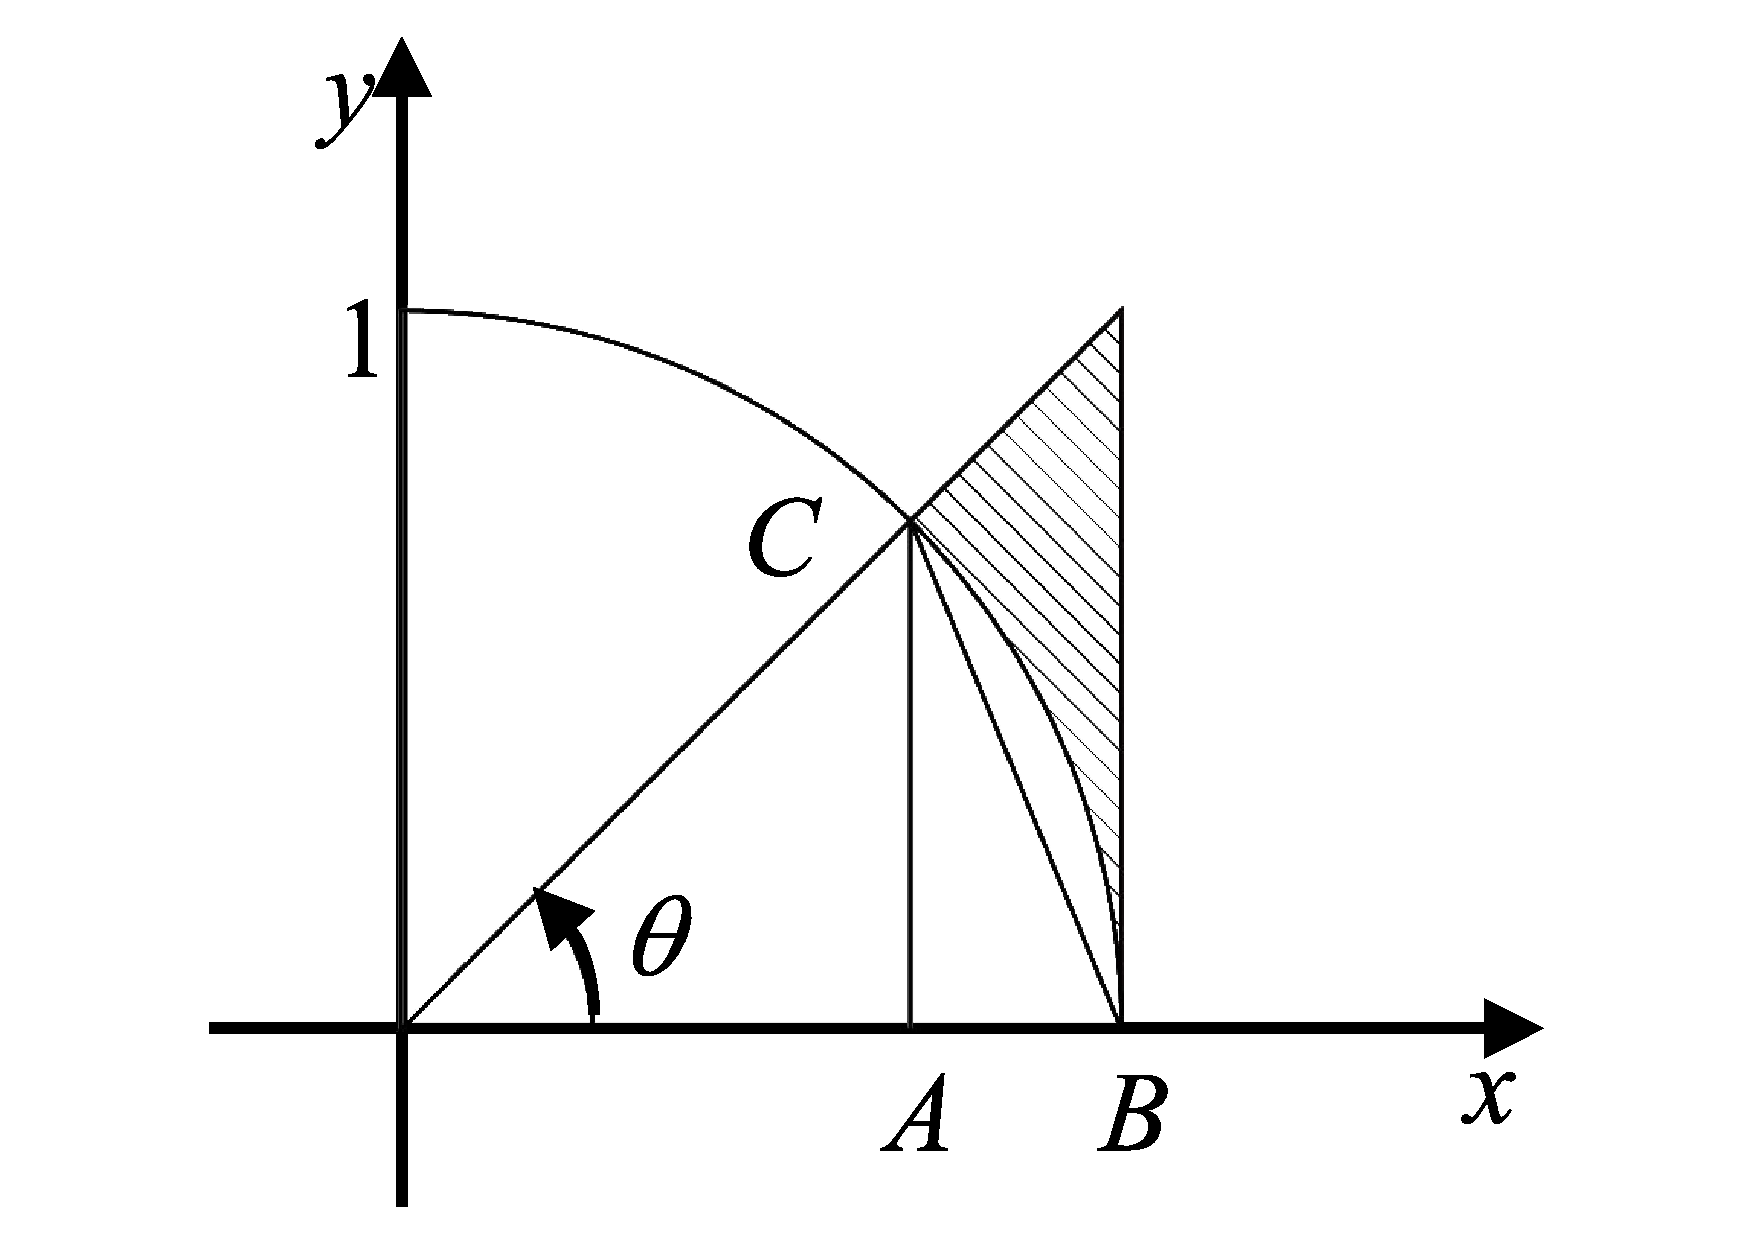
\includegraphics[width=4cm]{2012-figure.pdf} % 引入图片源
      \end{figure} % 图片结束
      \vspace{-1em}

    \item 证明当$n$充分大时，$\left(\sqrt[n]{n}-1\right)^{\frac{1}{n}}\left(
      \sqrt{1+\frac{1}{n^{2}}}-1\right)<\frac{1}{n^{2}}$.
      \vspace{10em}

    \item 若$\lim_{n\to\infty}x_{n}=a$，$\lim_{n\to\infty}y_{n}=b$，且$a<b$，依据极限定义证明当$n$充分大时，$x
      _{n}<y_{n}$.
      \vspace{9em}

    \item 设物体$P$沿抛物线$x=y^{2}(y>0)$自原点向右移动，与原点的距离为$r$.设其水平速度$\frac{\mathrm{d}x}{\mathrm{d}t}$保持为常量$A$.

      （1）计算$\frac{\mathrm{d}r}{\mathrm{d}t}$.

      （2）随着物体的移动，$\frac{\mathrm{d}r}{\mathrm{d}t}$是逐渐变大还是逐渐变小或者忽大忽小？

      （3）计算$\frac{\mathrm{d}r}{\mathrm{d}t}$的最终极限.
      \vspace{11em}
  \end{enumerate}

  \section{证明题(每小题 6 分，共 12 分)}
  \begin{enumerate}
    \setcounter{enumi}{16}
    \item 设$f(x)$在$[a,b]$上连续，在$(a,b)$内可导，且$f'(x)\neq0$.试证存在$\xi
      ,\eta\in(a,b)$，使得
      \[
        \frac{f'(\xi)}{f'(\eta)}=\frac{\mathrm{e}^{b}-\mathrm{e}^{a}}{b-a}\mathrm{e}
        ^{-\eta}.
      \]
      \vspace{12em}

    \item 设$f(x)$在闭区间$[0,1]$上连续，$f(0)=f(1)$，证明存在$x_{0}\in[0,1]$，使得$f
      (x_{0})=f\left(x_{0}+\frac{1}{4}\right)$.
      \vspace{12em}
  \end{enumerate}

  \chapter{2012-2013学年微积分（一）（上）期中考试参考答案}
  \section{基本计算题(每小题 5 分，共 60 分)}
  \begin{enumerate}
    \item \textbf{Solution}. $\frac{n}{n+\sqrt{n}}<\frac{1}{n+1}+\frac{1}{n+\sqrt{2}}
      +\cdots+\frac{1}{n+\sqrt{n}}<\frac{n}{n+1}$.

      因为$\lim_{n\to\infty}\frac{n}{n+\sqrt{n}}=\lim_{n\to\infty}\frac{n}{n+1}=1$，由夹逼定理得$l
      =1$.

    \item \textbf{Solution}.
      \[
        \begin{aligned}
          l = & \lim_{x\to \pi^+}\frac{\sqrt{2\cos^2 \frac{x}{2}}}{\sin x}=\lim_{x\to\pi^+}\frac{\sqrt{2}\left|\cos\frac{x}{2}\right|}{\sin x} \\
          =   & \lim_{x\to\pi^+}\frac{-\sqrt{2}\cos\frac{x}{2}}{2\sin \frac{x}{2}\cos \frac{x}{2}}                                             \\
          =   & -\frac{\sqrt{2}}{2}.
        \end{aligned}
      \]

    \item \textbf{Solution}.
      \[
        \begin{aligned}
          l= & \exp\left\{\lim_{x\to0}\frac{1}{\mathrm{e}^x-1}\left[\frac{\ln(1+x)}{x}-1\right]\right\}                              \\
          =  & \exp\left[\lim_{x\to0}\frac{\ln(1+x)-x}{x^2}\right]=\exp\left[\lim_{x\to0}\frac{x-\frac{x^2}{2}+o(x^2)-x}{x^2}\right] \\
          =  & \frac{1}{\sqrt{e}}.
        \end{aligned}
      \]

    \item \textbf{Solution}.
      \[
        \begin{aligned}
          l = & \lim_{x\to0}\frac{\left(\sqrt{1+2x}-1-x\right)\left(\sqrt{1+2x}+1+x\right)}{x^2\left(\sqrt{1+2x}+1+x\right)}=\lim_{x\to0}\frac{1+2x-(1+x)^2}{x^2\left(\sqrt{1+2x}+1+x\right)} \\
          =   & \lim_{x\to0}\frac{1+2x-1-2x-x^2}{x^2\left(\sqrt{1+2x}+1+x\right)}=-\frac{1}{2}.
        \end{aligned}
      \]

    \item \textbf{Solution}.
      \[
        \begin{aligned}
          f'(1) = & \lim_{x\to1}\frac{f(x)-f(1)}{x-1}                                        \\
          =       & \lim_{x\to1}\frac{(x-1)(x-2)\cdots(x-100)}{(x+1)(x+2)\cdots(x+100)(x-1)} \\
          =       & \lim_{x\to1}\frac{(x-2)\cdots(x-100)}{(x+1)(x+2)\cdots(x+100)}           \\
          =       & \frac{(-1)^{99}\cdot 99!}{101!}=-\frac{1}{10100}.
        \end{aligned}
      \]

    \item \textbf{Solution}.
      \[
        \begin{aligned}
          f'(x) = & \left[\frac{1}{2}\ln\left(x+\sqrt{x+\sqrt{x+1}}\right)\right]'                                                                  \\
          =       & \frac{1}{2\left(x+\sqrt{x+\sqrt{x+1}}\right)}\left(x+\sqrt{x+\sqrt{x+1}}\right)'                                                \\
          =       & \frac{1}{2\left(x+\sqrt{x+\sqrt{x+1}}\right)}\left[1+\frac{1}{2\sqrt{x+\sqrt{x+1}}}\left(1+\frac{1}{2\sqrt{x+1}}\right)\right].
        \end{aligned}
      \]

      将$x=0$代入上式得$f'(0)=\frac{1}{2}\left(1+\frac{1}{2}\cdot\frac{3}{2}\right
      )=\frac{7}{8}$.

    \item \textbf{Solution}. 取对数，得$\ln x + f(y) = y\ln x + \ln\ln 3$.方程两边微分得
      \[
        \frac{1}{x}\mathrm{d}x + f'(y)\mathrm{d}y = \ln x \mathrm{d}y + y\cdot\frac{1}{x}
        \mathrm{d}x.
      \]

      整理得$\mathrm{d}y=\frac{y-1}{x\left[f'(y)-\ln x\right]}\mathrm{d}x$.

    \item \textbf{Solution}. $\frac{\mathrm{d}y}{\mathrm{d}x}=\frac{\frac{\mathrm{d}y}{\mathrm{d}t}}{\frac{\mathrm{d}x}{\mathrm{d}t}}
      =\frac{mt^{m-1}}{\frac{2}{2t}}=mt^{m}$，

      $\frac{\mathrm{d}^{2}y}{\mathrm{d}x^{2}}=\frac{\mathrm{d}}{\mathrm{d}t}\left
      (\frac{\mathrm{d}y}{\mathrm{d}x}\right)\cdot\frac{\mathrm{d}t}{\mathrm{d}x}
      =\left(mt^{m}\right)'_{t}\cdot\frac{1}{\frac{1}{t}}=m^{2} t^{m}$.

      设$\frac{\mathrm{d}^{k} y}{\mathrm{d}x^{k}}=m^{k} t^{m}$，则$\frac{\mathrm{d}^{k+1}y}{\mathrm{d}x^{k+1}}
      =\frac{\mathrm{d}}{\mathrm{d}t}\left (\frac{\mathrm{d}^{k} y}{\mathrm{d}x^{k}}
      \right)\cdot\frac{\mathrm{d}t}{\mathrm{d}x}=\left(m^{k} t^{m}\right)'\cdot\frac{1}{\frac{1}{t}}
      =m^{k+1}t^{m}$.

      由数学归纳法得$\frac{\mathrm{d}^{n} y}{\mathrm{d}x^{n}}=m^{n} t^{m}$，所以$\left
      .\frac{\mathrm{d}^{n} y}{\mathrm{d}x^{n}}\right|_{t=1}=m^{n}$.

    \item \textbf{Solution}.
      \[
        u = \sqrt[3]{1-x+x^{2}-x^{3}}-1 = 1+\frac{1}{3}(-x+x^{2}-x^{3})+o(-x+x^{2}
        -x^{3})-1=-\frac{1}{3}x+o(x).
      \]

      所以$u\sim -\frac{1}{3}x$，即$c=-\frac{1}{3}$，$k=1$.

    \item \textbf{Solution}. $g(0)=0$，因$g'_{-}(0)=\lim_{x\to0^-}\frac{g(x)-g(0)}{x}
      =\lim_{x\to0^-}\arctan \frac{1}{x}=-\frac{\pi}{2}=g'_{+}(0)=b$，所以$b=-\frac{\pi}{2}$.

      $\left.\frac{\mathrm{d}}{\mathrm{d}x}f\left(g(x)\right)\right|_{x=0}=f'(g(0
      ))\cdot g'(0)=\cos 0 \cdot b=-\frac{\pi}{2}$.

    \item \textbf{Solution}. $f(x)=\frac{1}{2x-1}+\frac{1}{x+1}$，所以
      \[
        f^{(n)}(0)=\left.\frac{(-1)^{n}\cdot n!\,2^{n}}{(2x-1)^{n+1}}\right|_{x=0}
        +\left.\frac{(-1)^{n}\cdot n!}{(x+1)^{n+1}}\right|_{x=0}=n!\left[(-1)^{n}
        -2^{n}\right].
      \]

    \item \textbf{Solution}. 当$|x|>1$时，$x^{n}\to\infty$，所以$f(x)=\lim_{n\to\infty}
      \frac{x^{n}}{1+x^{n}}=1$；

      当$x=1$时，$f(x)=\frac{1}{2}$；当$x=-1$时，$f(x)$不存在；

      当$|x|<1$时，$x^{n}\to0$，所以$f(x)=\lim_{n\to\infty}\frac{x^{n}}{1+x^{n}}=
      0$.

      综上所述，$f(x)=
      \begin{cases}
        1,           & |x|>1, \\
        \frac{1}{2}, & x=1,   \\
        \text{不存在},  & x=-1,  \\
        0,           & |x|<1.
      \end{cases}$

      $f(x)$的间断点为$x=-1$和$x=1$.

      因为$f(1^{-})=0$，$f(1^{+})=1$，$f(-1^{-})=1$，$f(-1^{+})=0$，所以$x=1$和$x
      =-1$都是跳跃间断点.
  \end{enumerate}

  \section{综合题(每小题 7 分，共 28 分)}
  \begin{enumerate}
    \setcounter{enumi}{12}
    \item \textbf{Solution}. 由几何关系，$a(\theta)=\frac{1}{2}\sin\theta(1-
      \cos\theta)$，$b(\theta)=\frac{1}{2}\tan\theta-\frac{1}{2}\theta$.

      当$\theta\to0$时，$a(\theta)\to0$，$b(\theta)\to0$，所以$a(\theta)$和$b(\theta
      )$都是无穷小.计算
      \[
        \begin{aligned}
          \lim_{\theta\to0}\frac{a(\theta)}{b(\theta)}= & \lim_{\theta\to0}\frac{\sin\theta(1-\cos\theta)}{\tan\theta-\theta}                                                         \\
          =                                             & \frac{1}{2}\lim_{\theta\to0}\frac{\theta^3}{\tan\theta-\theta}=\frac{1}{2}\lim_{\theta\to0}\frac{3\theta^2}{\sec^2\theta-1} \\
          =                                             & \frac{3}{2}\lim_{\theta\to0}\frac{\theta^2}{\tan^2\theta}=\frac{3}{2}.
        \end{aligned}
      \]

      所以当$\theta\to0$时，$a(\theta)$与$b(\theta)$是同阶无穷小.

    \item \textbf{Solution}. 计算
      \[
        \begin{aligned}
          \lim_{x\to+\infty}\frac{\left(\sqrt[x]{x}-1\right)^{\frac{1}{x}}\left(\sqrt{1+\frac{1}{x^2}}-1\right)}{\frac{1}{x^2}}= & \lim_{x\to+\infty}\left(\sqrt[x]{x}-1\right)^{\frac{1}{x}}\cdot\lim_{x\to+\infty}\frac{\frac{1}{2x^2}+o\left(\frac{1}{x^2}\right)}{\frac{1}{x^2}}                                                                                              \\
          =                                                                                                                      & \frac{1}{2}\lim_{x\to+\infty}\left(\sqrt[x]{x}-1\right)^{\frac{1}{x}}=\frac{1}{2}\lim_{x\to+\infty}\left(\mathrm{e}^{\frac{\ln x}{x}}-1\right)^{\frac{1}{x}}                                                                                   \\
          =                                                                                                                      & \frac{1}{2}\exp\left[\lim_{x\to+\infty}\frac{\ln\left(\mathrm{e}^{\frac{\ln x}{x}}-1\right)}{x}\right]                                                                                                                                         \\
          =                                                                                                                      & \frac{1}{2}\exp\left[\lim_{x\to+\infty}\frac{\mathrm{e}^{\frac{\ln x}{x}}\cdot\frac{1-\ln x}{x^2}}{\mathrm{e}^{\frac{\ln x}{x}}-1}\right] = \frac{1}{2}\exp\left[\lim_{x\to+\infty}\frac{\mathrm{e}^{\frac{\ln x}{x}}(1-\ln x)}{x\ln x}\right] \\
          =                                                                                                                      & \frac{1}{2}\exp\left[\lim_{x\to+\infty}\frac{1-\ln x}{x\ln x}\right] = \frac{1}{2}\exp\left[\lim_{x\to+\infty}\frac{\frac{1}{\ln x}-1}{x}\right]=\frac{1}{2}.
        \end{aligned}
      \]

      所以$\lim_{n\to\infty}\frac{\left(\sqrt[n]{n}-1\right)^{\frac{1}{n}}\left(\sqrt{1+\frac{1}{n^2}}-1\right)}{\frac{1}{n^{2}}}
      =\frac{1}{2}<1$，

      由极限的保号性，当$n$充分大时，有$\left(\sqrt[n]{n}-1\right)^{\frac{1}{n}}\left
      (\sqrt{1+\frac{1}{n^{2}}}-1\right)<\frac{1}{n^{2}}$.

    \item \textbf{Solution}. 对于$\varepsilon=\frac{b-a}{2}>0$，

      由极限的定义，存在$N_{1}$使得当$n>N_{1}$时，$|x_{n}-a|<\varepsilon$；存在$N
      _{2}$使得当$n>N_{2}$时，$|y_{n}-b|<\varepsilon$.

      设$N=\max\{N_{1},N_{2}\}$，则当$n>N$时，$x_{n}<a+\varepsilon=\frac{a+b}{2}<
      b-\varepsilon<y_{n}$.

    \item \textbf{Solution}. （1）由题设$r=\sqrt{x^{2}+y^{2}}=\sqrt{x^{2}+x}$，所以$\frac{\mathrm{d}r}{\mathrm{d}t}
      =\frac{2x+1}{2\sqrt{x^{2}+x}}\cdot\frac{\mathrm{d}x}{\mathrm{d}t}=\frac{(2x+1)A}{2\sqrt{x^{2}+x}}$.

      （2）
      \[
        \begin{aligned}
          \frac{\mathrm{d}^2 r}{\mathrm{d}t^2}= & \frac{\mathrm{d}}{\mathrm{d}x}\left[\frac{(2x+1)A}{2\sqrt{x^2+x}}\right]\cdot\frac{\mathrm{d}x}{\mathrm{d}t}    \\
          =                                     & \frac{1}{2}\cdot\frac{2\sqrt{x^2+x}-\frac{(2x+1)^2}{2\sqrt{x^2+x}}}{x^2+x}\cdot A^{2}                           \\
          =                                     & \frac{1}{2}\cdot\frac{4(x^2+x)-(2x+1)^2}{2(x^2+x)\sqrt{x^2+x}}\cdot A^{2} = -\frac{A^2}{(x^2+x)\sqrt{x^2+x}}<0.
        \end{aligned}
      \]

      所以$\frac{\mathrm{d}r}{\mathrm{d}t}$逐渐变小.

      （3）$\lim_{x\to+\infty}\frac{\mathrm{d}r}{\mathrm{d}t}=\lim_{x\to+\infty}\frac{(2x+1)A}{2\sqrt{x^{2}+x}}
      =A$.
  \end{enumerate}

  \section{证明题(每小题 6 分，共 12 分)}
  \begin{enumerate}
    \setcounter{enumi}{16}
    \item \textbf{Proof}.函数$f(x)$和函数$y=\mathrm{e}^{x}$均在$[a,b]$上连续，在$(
      a,b)$内可导，且$\mathrm{e}^{x}\neq0$.

      由Cauchy中值定理，存在$\eta\in(a,b)$使得
      \[
        \frac{f(b)-f(a)}{\mathrm{e}^{b}-\mathrm{e}^{a}}=\frac{f'(\eta)}{\mathrm{e}^{\eta}}
        .
      \]

      对函数$f(x)$应用Lagrange中值定理，存在$\xi\in(a,b)$使得$f(b)-f(a)=f'(\xi)(b
      -a)$，

      代入上式即得$\frac{f'(\xi)}{f'(\eta)}=\frac{\mathrm{e}^{b}-\mathrm{e}^{a}}{b-a}
      \mathrm{e}^{-\eta}$.

    \item \textbf{Proof}. 令$F(x)=f(x)-f\left(x+\frac{1}{4}\right)$，显然$F(
      x)$在$\left[0,\frac{3}{4}\right]$上连续.

      注意到
      \[
        \begin{aligned}
          \frac{F(0)+F\left(\frac{1}{4}\right)+F\left(\frac{2}{4}\right)+F\left(\frac{3}{4}\right)}{4}= & \frac{1}{4}\left[f(0)-f\left(\frac{1}{4}\right)+f\left(\frac{1}{4}\right)-f\left(\frac{2}{4}\right)+f\left(\frac{2}{4}\right)-f\left(\frac{3}{4}\right)+f\left(\frac{3}{4}\right)-f(1)\right] \\
          =                                                                                             & \frac{1}{4}\left[f(0)-f(1)\right]=0.
        \end{aligned}
      \]

      由介值定理，存在$x_{0}\in\left[0,\frac{3}{4}\right]\subset[0,1]$，使得$F(x_{0}
      )=0$，即$f(x_{0})=f\left(x_{0}+\frac{1}{4}\right)$.
  \end{enumerate}
\end{document}
